Section{Introduction} 
The website we are designing is about the 2014 Austin City Limits (ACL) music festival. The website design has three main pages: Artists, Stages, and Sponsors.
The website allows anyone to view pages about current Artists, Sponsors, and Stages. The technologies used are PythonAnywhere, Python 3.4, Django 1.6,
Twitter Bootstrap 3.2, Apiary, and the database sqlite3. PythonAnywhere is used to host the site using the Django web-framework to 
construct the necessary models and views to handle HTTP requests. Twitter Bootstrap is used to organize common data among different
types of pages into a base template HTML file. <!--EDIT:STEPHEN--> Customizations to the HTML and Twitter Bootstrap designs are made through
the use of a custom CSS file.

The database we chose to test with (see Tests) is sqlite3. We currently don't use it to load any data to render the HTML pages.

\section{Design}
Our current design of the website uses HTML and Twitter Bootstrap to stylize each page and PythonAnywhere to host the page. 
Using Django's templating language we are able to reuse html files by extending from them. Currently we only have a single base html page that
uses Twitter Bootstrap. We have nine pages in static HTML that provide examples of the web page design and content. <!--EDIT:STEPHEN--> Each
page within a category (Artist,Sponsor,Stage) will link to the other two categories. Artists will link to Sponsors and Stages, Sponsors to
Artists and Stages, and Stages to Artists and Sponsors. In the future we are considering splitting Stages into two subcategories, Stages and
Events, which will incorporate the non-musical events within the Austin City Limits festival (Art Market, Food Court, Charity Events).

[UML model here]
\begin{figure}[h]
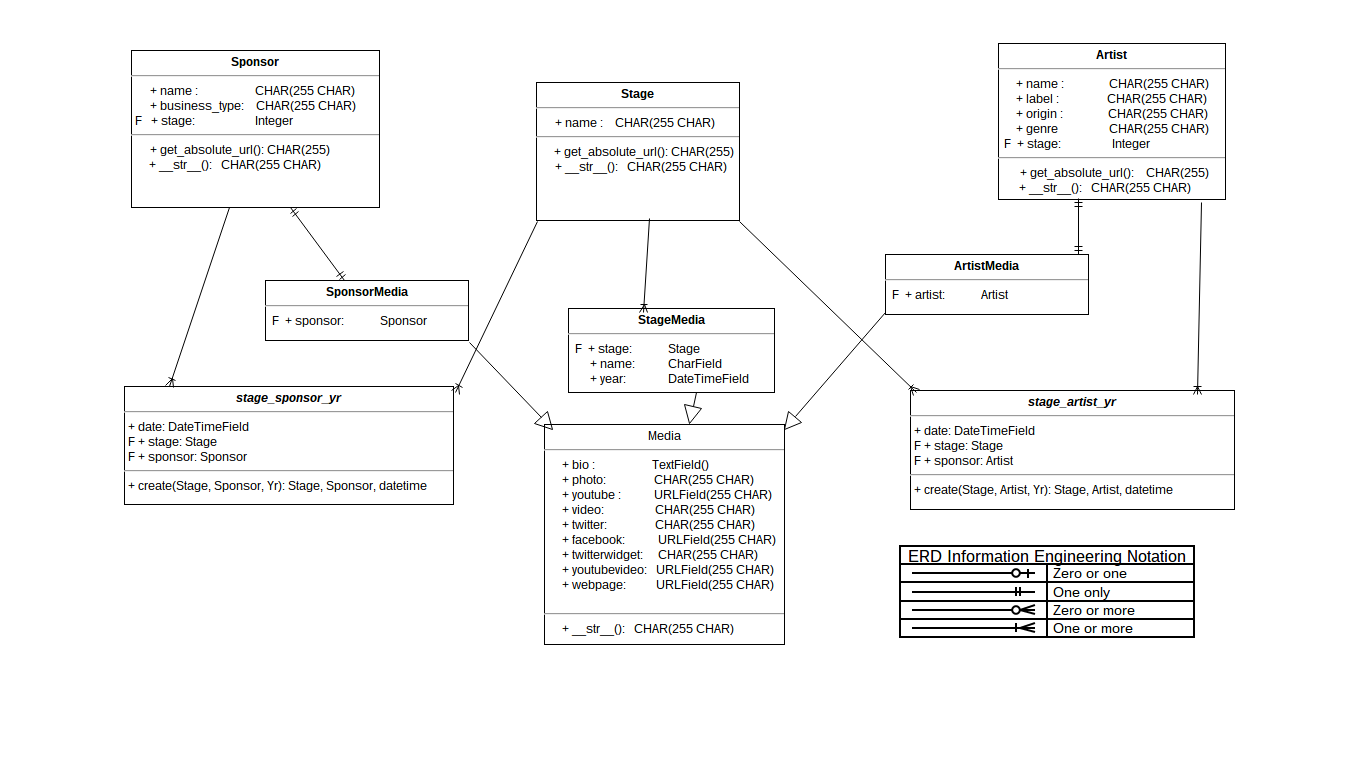
\includegraphics[width=\textwidth]{UML}
\end{figure}

\subsection{App Design}
The current directory structure on PythonAnywhere is outlined below for reference to files:

[tree -d layout here]

<!--EDIT BY STEPHEN-->
\subsection{Web Pages}
Each web page has basic information about a particular artist, sponsor, or stage involved in the ACL music festival.
Each page includes a bio, video, official website, Youtube channel, a Twitter feed, and Picture. All pages will include a navigation
bar at the top of their page that will allow the user to go back to the main "splash" page, as well as reach the Artists, Sponsors, and
Stages pages. In future phases we are considering incorporating a search bar inside of the navigation bar, so that the user can search 
all categories.

\subsection{Splash Page}
The "splash" page will be the first page a visitor to the site will see. It will provide button style links to all subcategories (Artists,
Sponsors, Stages).
\subsubsection{Artists}
Artist Pages can be reached from the home page as well as from the Stage or Sponsor pages depending on whether the Artist played on
a Stage that was hosted by a Sponsor. 
\subsubsection{Sponsors}
Sponsor pages can be reached from the home page as well as from the Artist or Stages pages depending on whether the Sponsor hosted a 
Stage, and that particular Artist played on that Stage.

\subsubsection{Stages}
Stages pages can be reached from the home page as well as from the Artist or Sponsor pages depending on whether the Sponsor hosted a 
Stage, and that particular Artist played on that Stage.
